\subsection{Non-Collision Backgrounds}
\label{sec:noncollision}

We estimate the rate of non-collision backgrounds which produce prompt photons using the ECAL timing variables for EM cluster. This estimate includes the contributions from ECAL “spikes”, as well as beam halo. To estimate these contribution we form crystal seed timing distributions of each background component i.e., spikes, beam halo and then fitted them to the candidate seed time distribution without shower shape or timing cuts to estimate how much each of these background contribute in the prompt region (  $|t_{seed} | < 3 $ns).

 The various templates are formed in the following way: 
    
\begin{itemize}
\item {\bf Candidate sample templates}: To construct the template for the candidate sample we apply cuts similar to our analysis cuts but with relaxed the shower shape variables and without offline R9 selection. We do not apply any fake E/T rejection cuts to increase the statistics in our templates. The distribution can be seen in Fig.\ref{fig:candidate}.
\item {\bf Prompt templates}: The templates for prompt events is made using the candidate sample in which the photon candidates are required to have a pixel seed match, as seen in Fig. ~\ref{fig:PromptTempl} .
\item {\bf Spikes templates}: The spike template is found by requiring one of the shower shape variables sihih 0.011 or sifif< 0.001 selection. These templates are shown in Fig. ~\ref{fig:SpikeTempl}.
\item {\bf Beam Halo templates}: The energy deposition from the beam halo muon could be reconstructed within the prompt window when the muon brems in the ECAL. To get the template of timing distributions of such objects, we apply similar cuts used for the candidate sample but require the MIP total energy to be greater than 4 GeV. The beam halo template is shown in Fig.~\ref{fig:beamhalo}. The MIP-tagging is a set of criteria developed in order to identify the passage of a beam halo muon across the acceptance of the ECAL. Crystals other than associated with EM shower  are identified along potential paths in a similar $\phi$ direction as of the seed crystal of EM shower, and then fitted with a straight line. The end results is the number of crystals associated along the selected trajectory, their total energy (MIP energy), and the $\chi^2$ of the fitted line. The beam hallo shower typicaly have more MIP energy than a true EM shower .
\end{itemize}



\begin{figure}[h]
\centering
{\label{fig:candidate}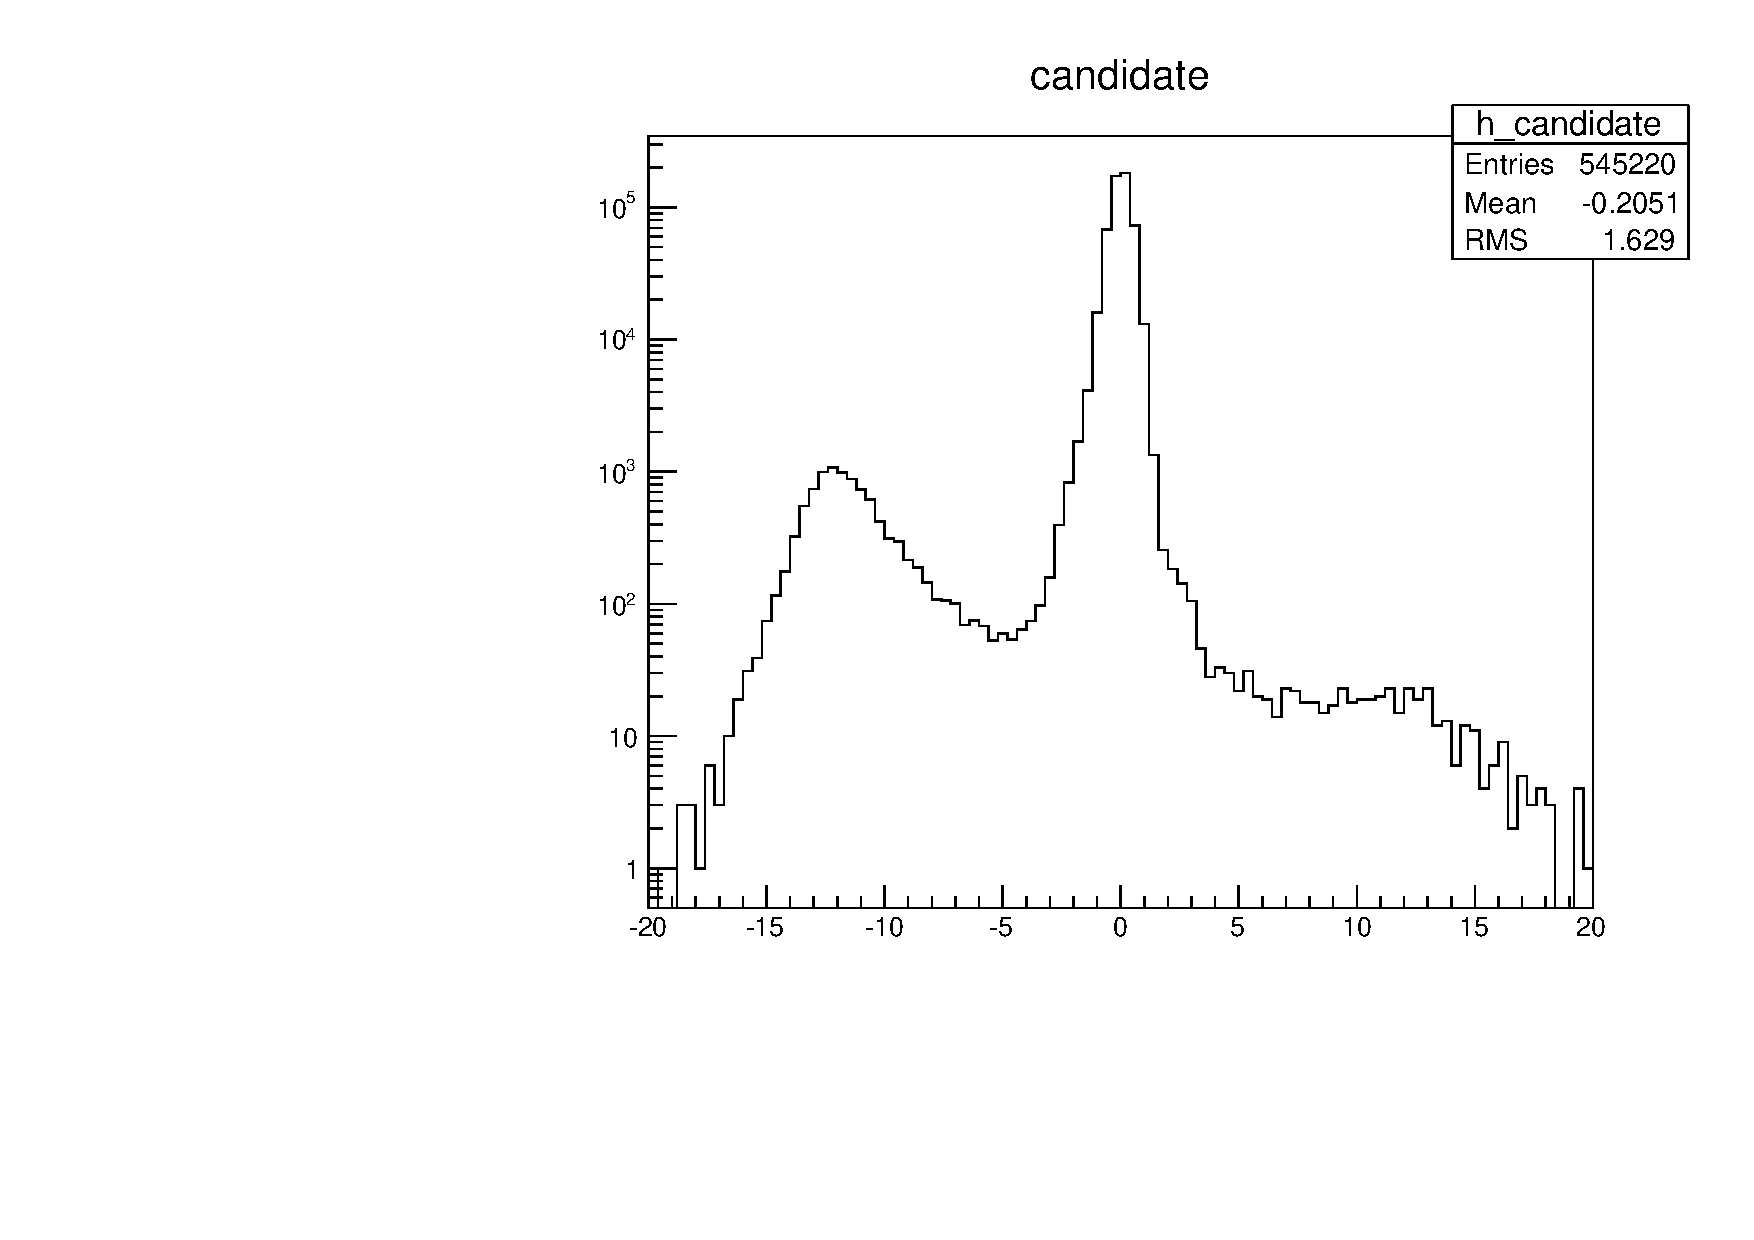
\includegraphics[width=0.45\textwidth]{analysis_figs/candidate_temp.pdf}}
{\label{fig:PromptTempl}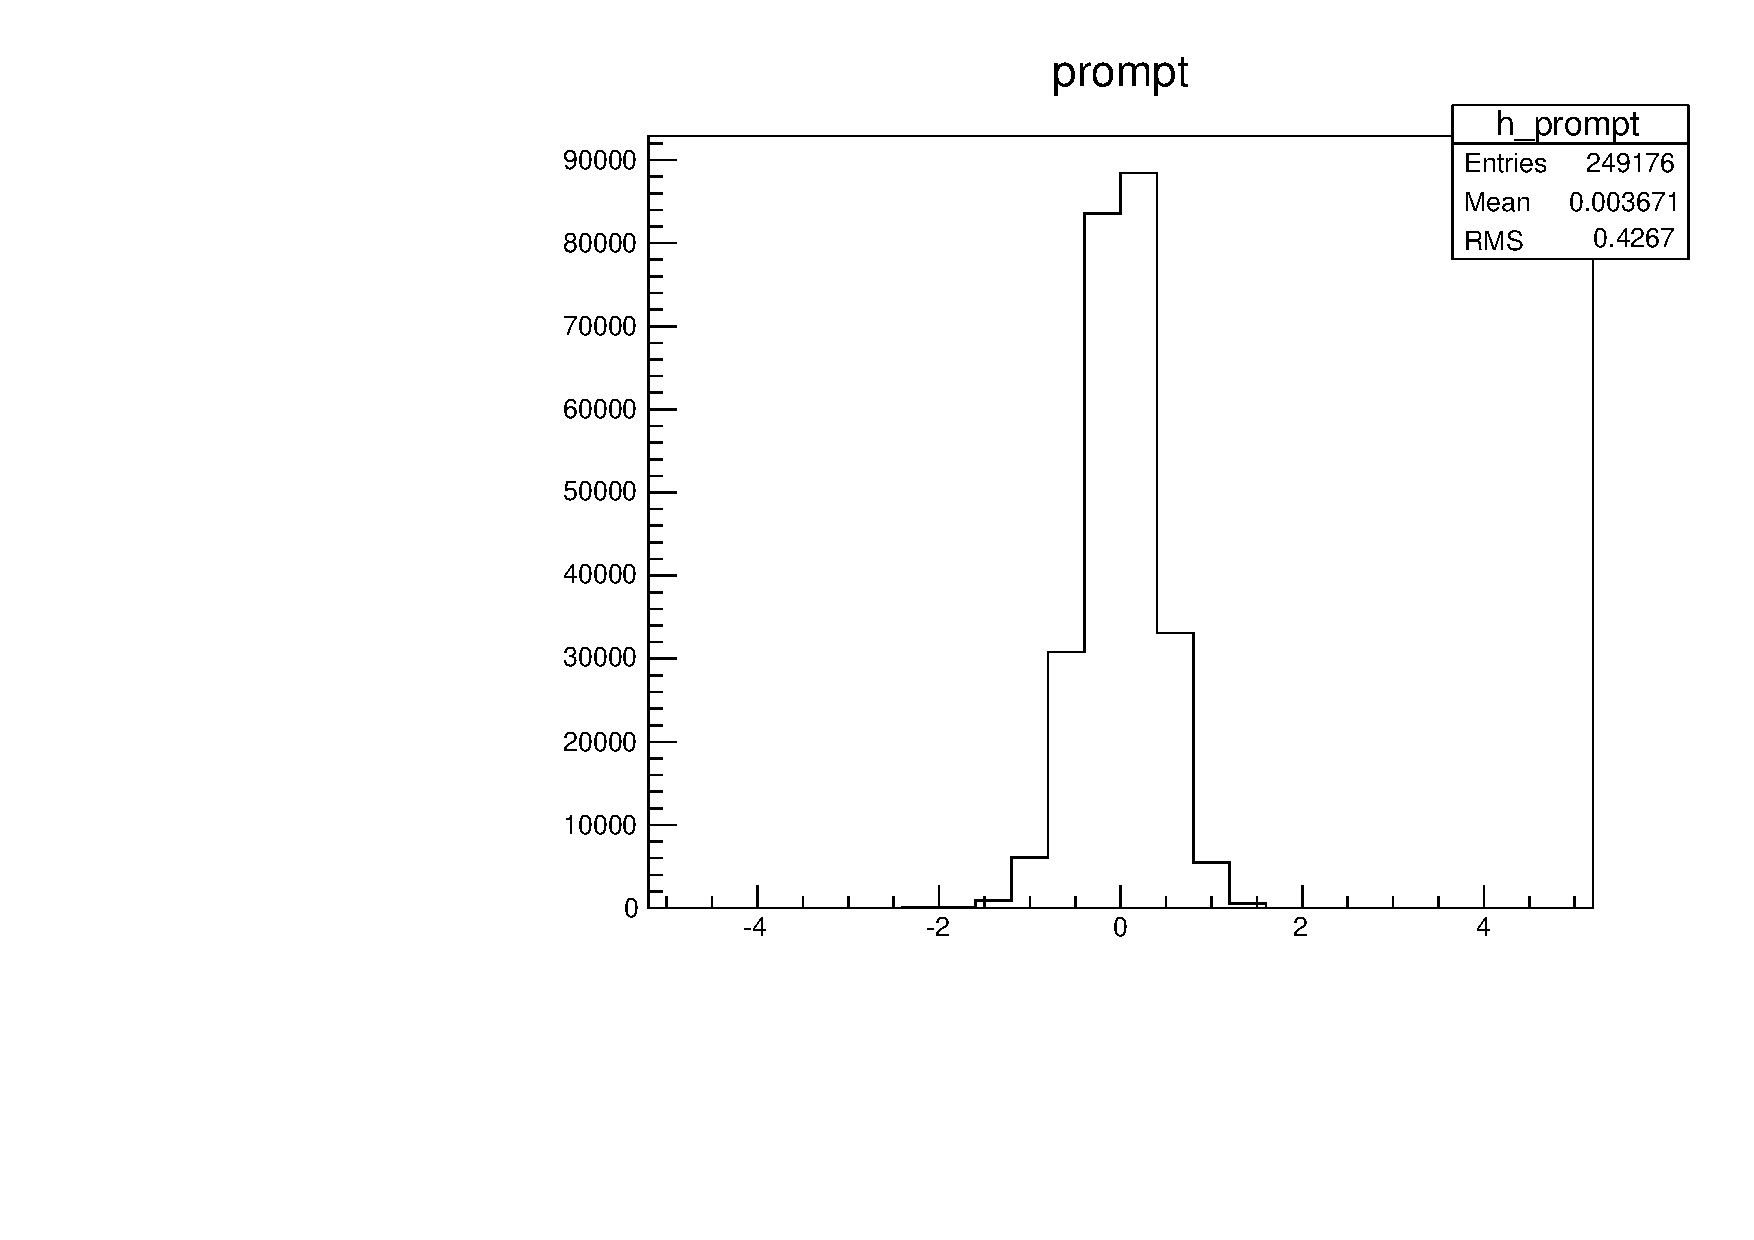
\includegraphics[width=0.45\textwidth]{analysis_figs/prompt.pdf}}
\caption{Seed time distribution (ns) for candidate events and prompt events.}
\end{figure}

\begin{figure}[h!]
\centering
{\label{fig:SpikeTempl}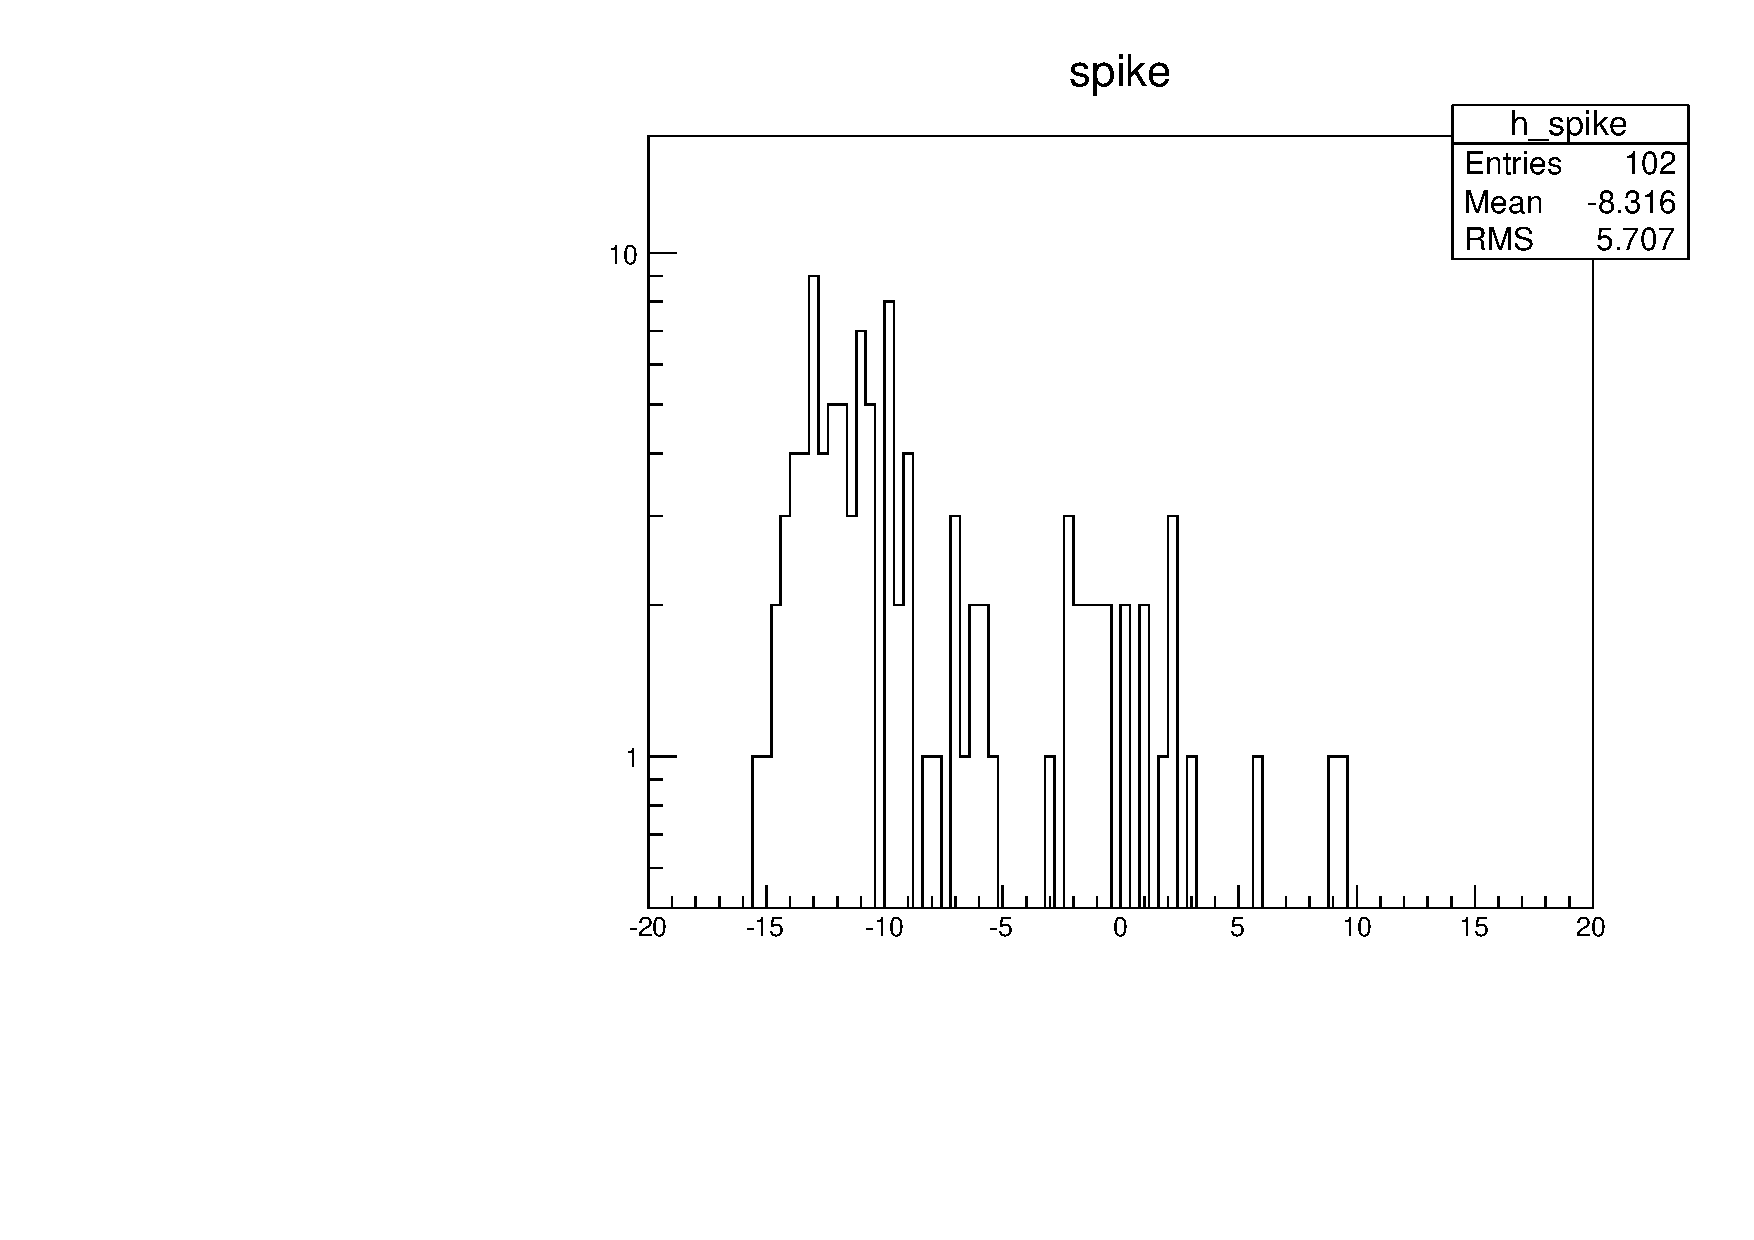
\includegraphics[width=0.45\textwidth]{analysis_figs/spike.pdf}}
{\label{fig:PromptTempl}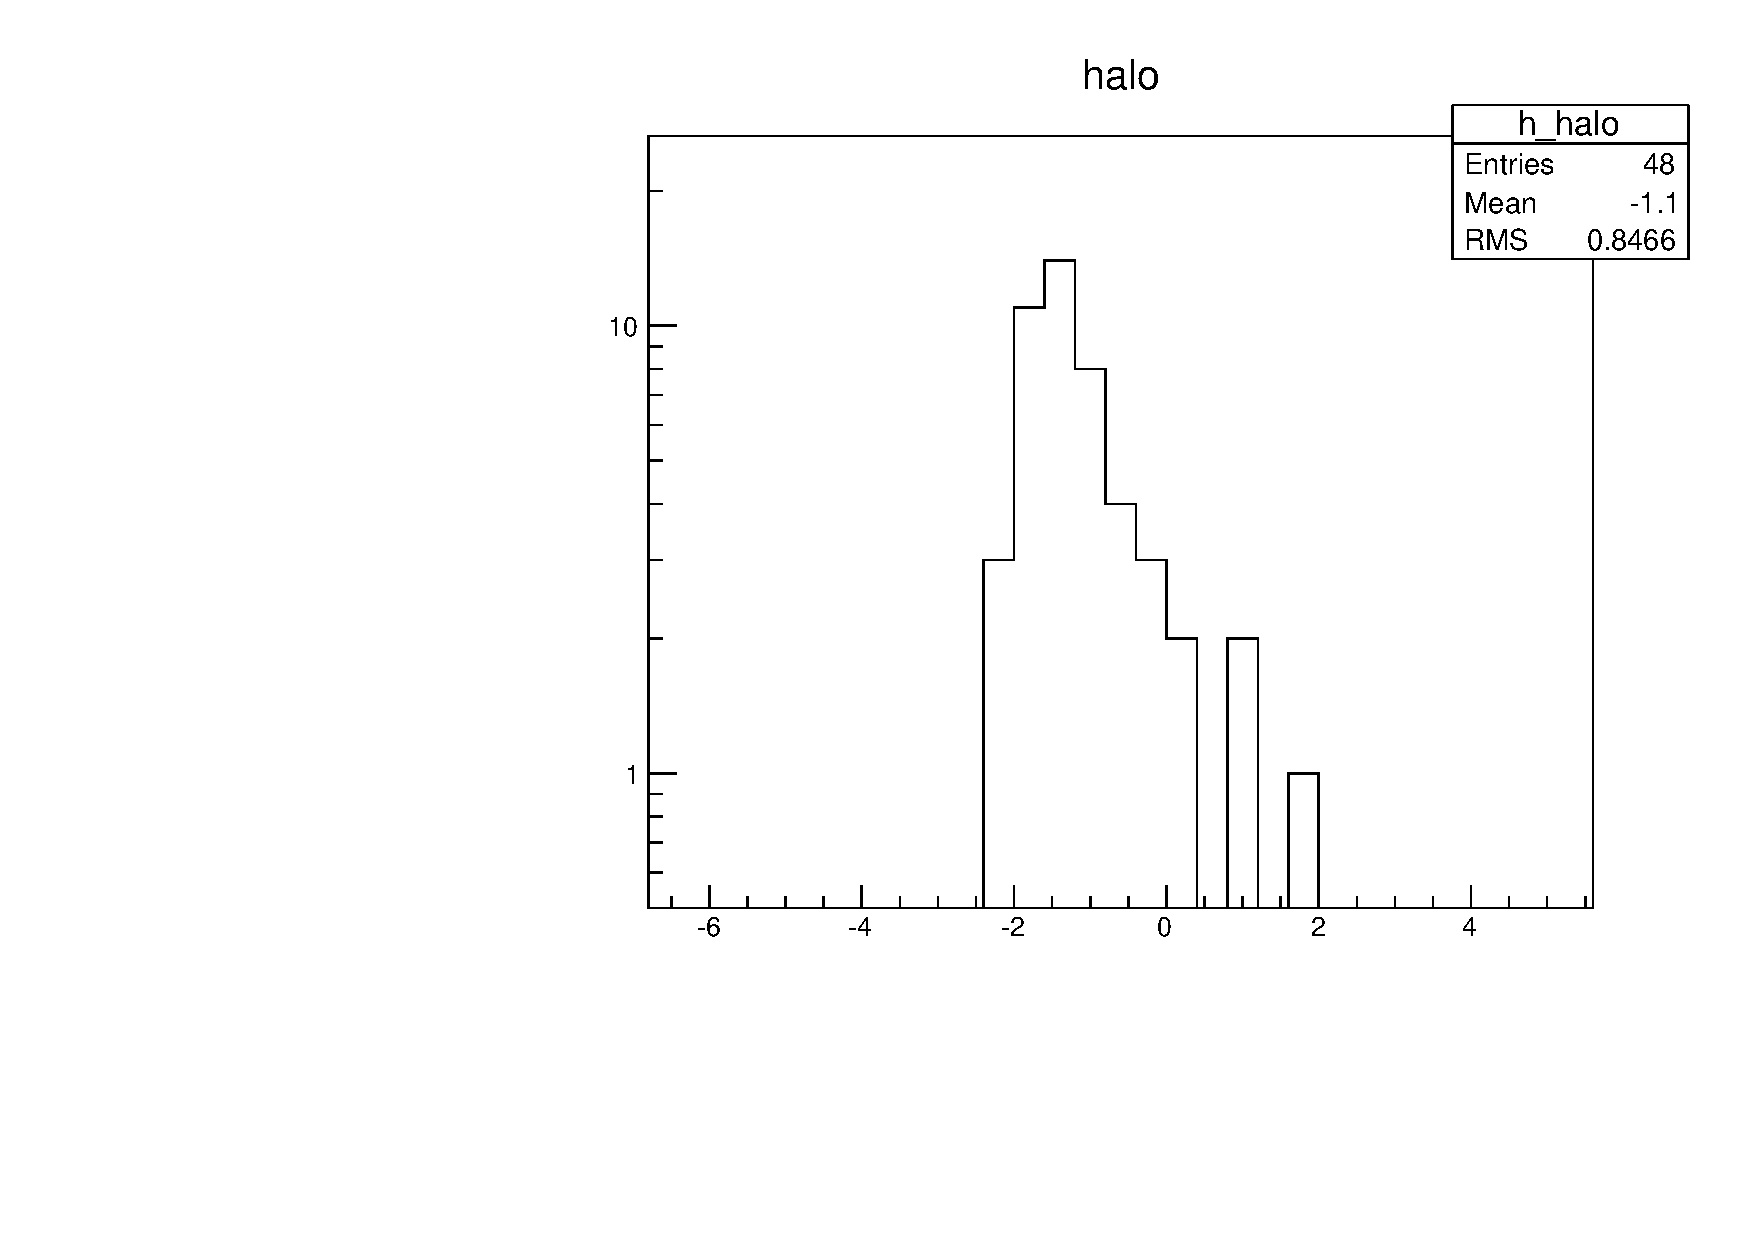
\includegraphics[width=0.45\textwidth]{analysis_figs/halo.pdf}}
\caption{Seed time distribution (ns) for spike and halo events}
\end{figure}

We estimate the final number of each non collision background events in data by the fitting the template distributions of spikes, beam halo and prompt to the complete timing distribution of the candidate events. Through this, we observe that the spike hypothesis is almost completely rejected, where the beam halo contribution is on the order of $< 1$ \% of the total expected events. Due to these results we have decided to neglect non-collision backgrounds in any further calculations.

\begin{figure}[h]
\centering
{\label{fig:can}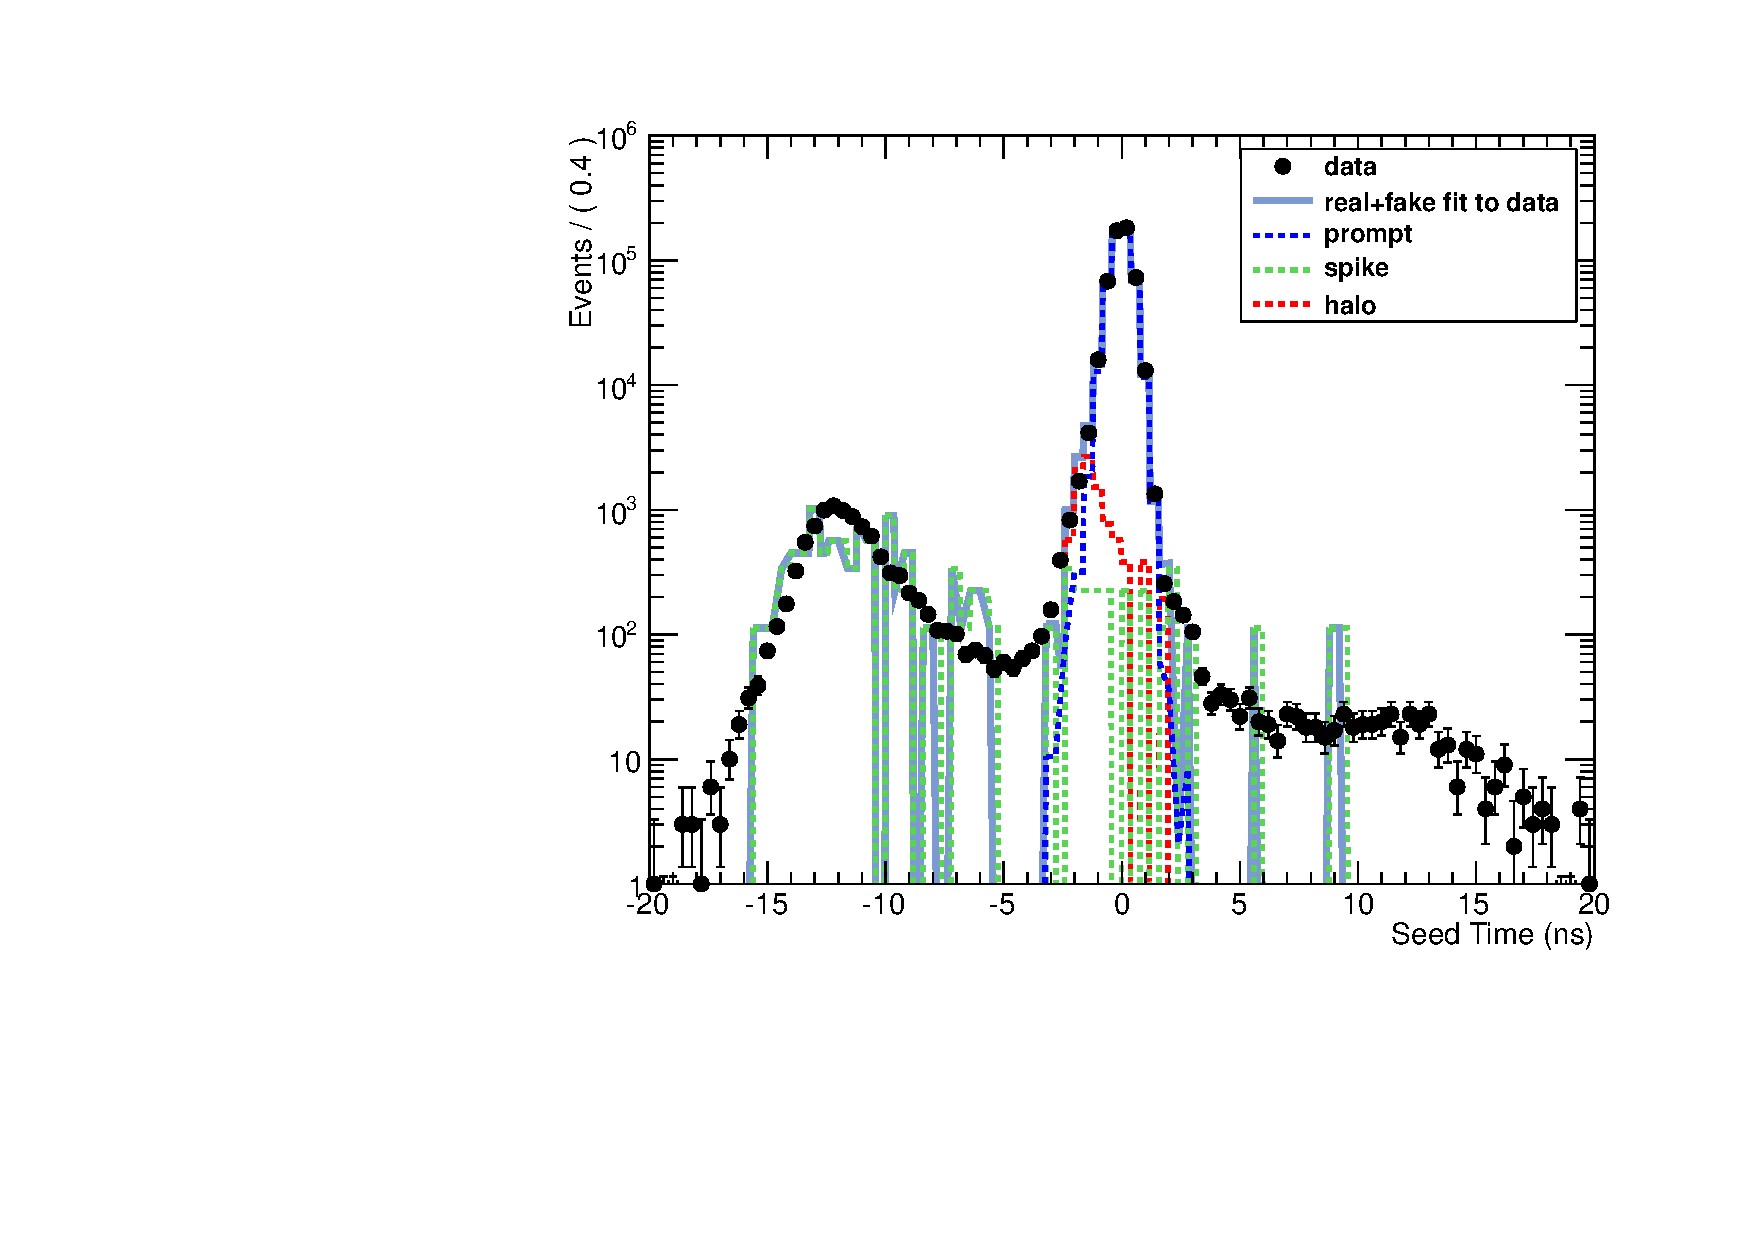
\includegraphics[width=0.45\textwidth]{analysis_figs/cadidate.pdf}}
{\label{fig:fit}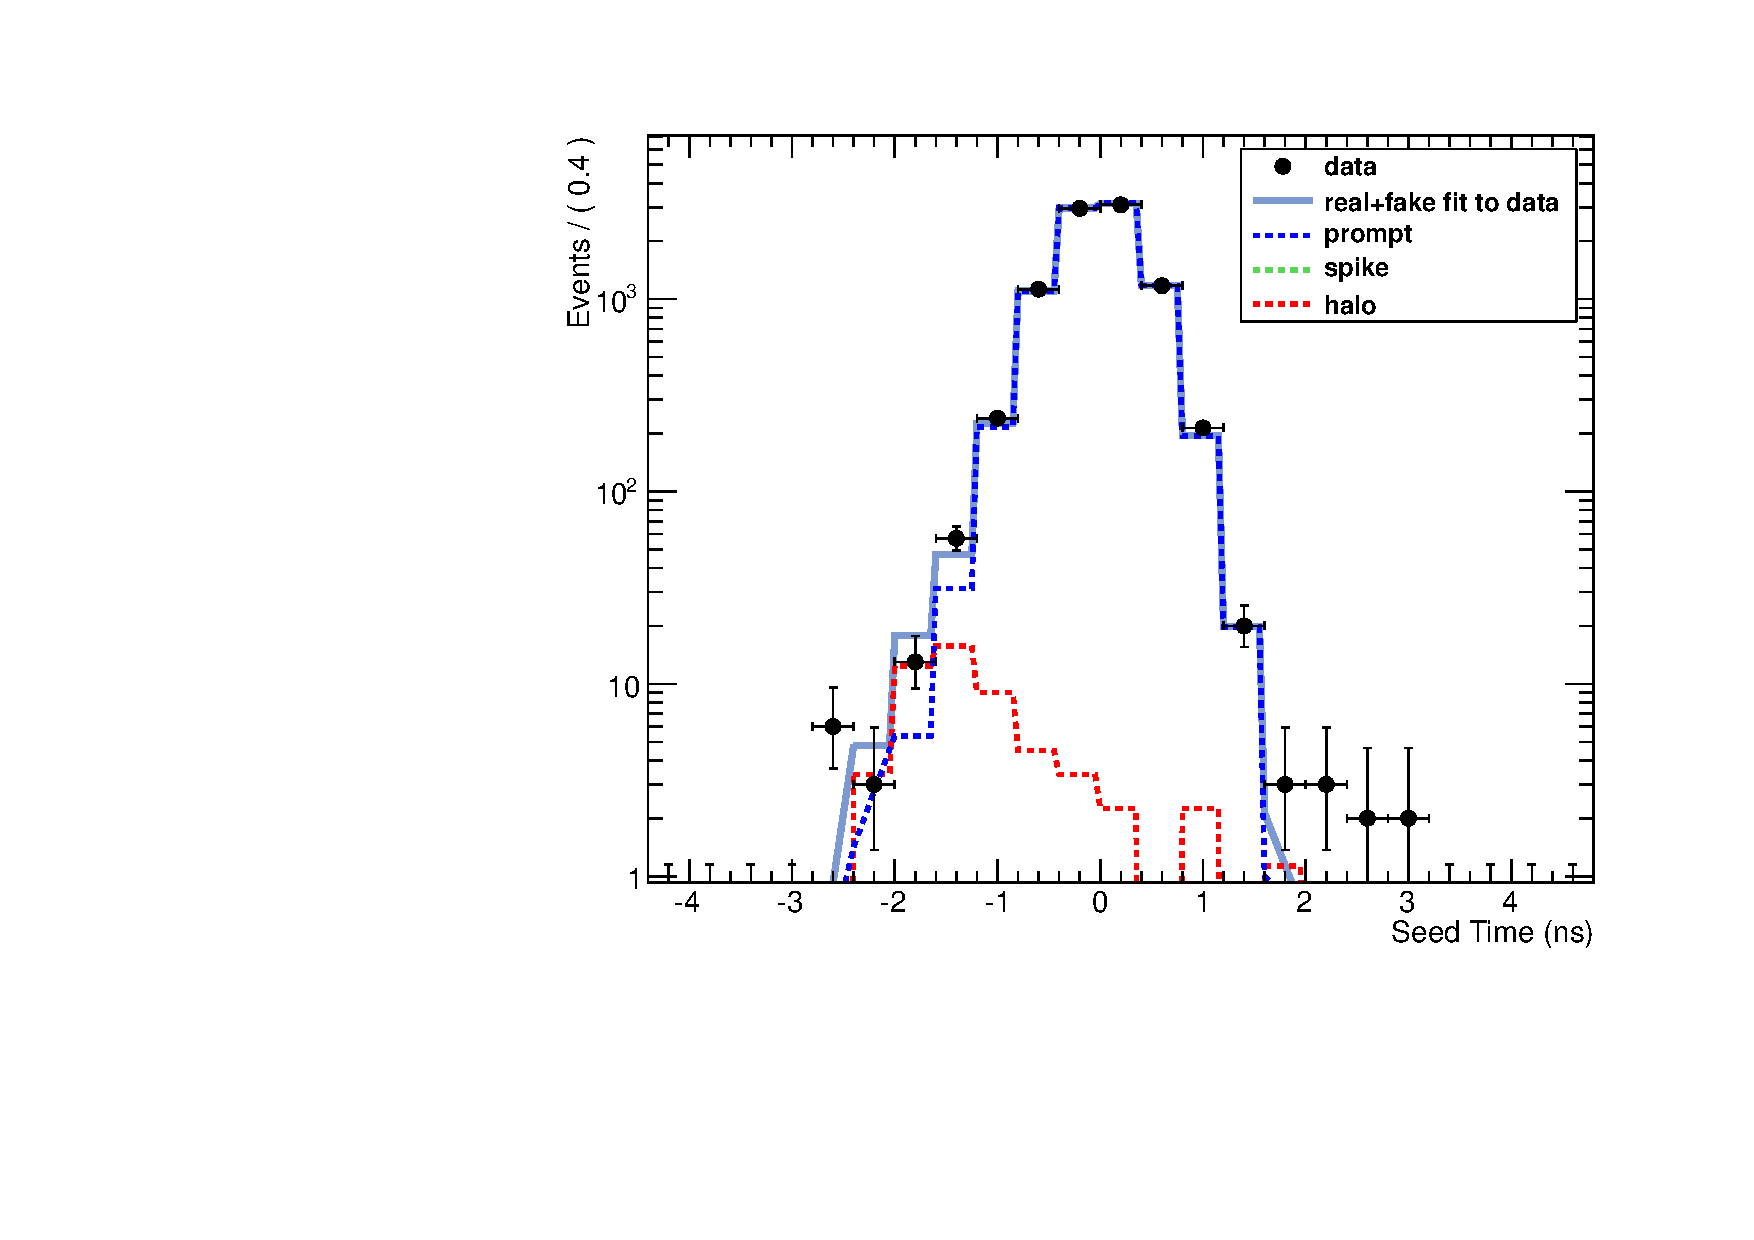
\includegraphics[width=0.45\textwidth]{analysis_figs/final_fit.pdf}}
\caption{Template fits to the candidate selectiona and model independent analysis selection.}
\label{fig:beamhalo}
\end{figure}
